\part{Instruction Level Parallelism}
\section{Pipelining}
El Pipeline es una técnica que permite superponer el procesamiento de múltiples instrucciones en una ejecución. Una vez que la primera instrucción fue fetcheada y pasa a la etapa de decodificación, se comienza a fetchear la siguiente instrucción. 

Bajo condiciones ideales y con un gran número de instrucciones, la mejora en velocidad de ejecución es directamente proporcional a la cantidad de etapas en el pipe. Es decir, un pipeline de 5 etapas, es aproximadamente 5 veces más rápido que el procesamiento secuencial.  

Si bien el pipelining reduce el tiempo de ejecución de un programa, debemos notar que no lo hace modificando el tiempo que se tarda en procesar una instrucción (\textbf{latency / latencia}) sino que aumenta la cantidad de instrucciones que se procesan por unidad de tiempo (\textbf{throughput}).
\begin{figure}[h]
	\centering
	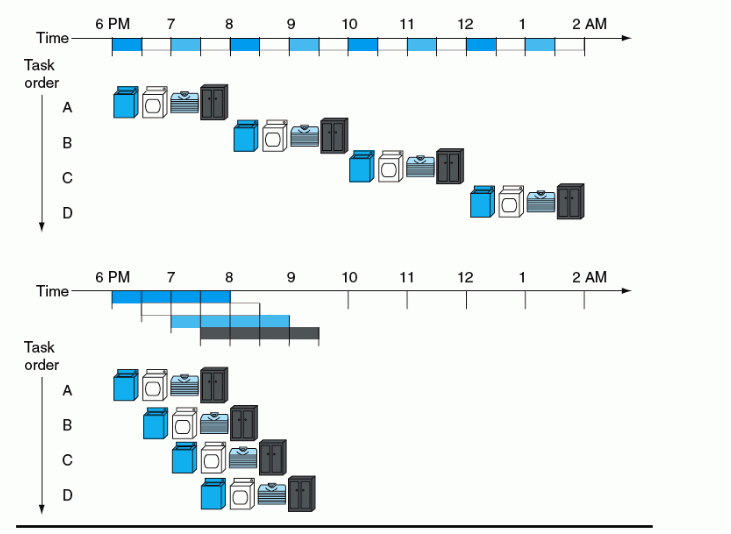
\includegraphics[width=0.5\linewidth]{imagenes/pipelining}
	\caption{Analogía de la lavandería: 4 personas tienen que lavar, secar, doblar y guardar su ropa sucia. Solo disponemos de una lavadora, una secadora, un ``doblador'' y un ropero. Si cada parte del proceso toma 30 minutos, y lo realizamos de manera secuencial, completarlo para las 4 personas tomaría ocho horas, mientras que si lo hacemos con un pipeline el tiempo se reduce a tres horas y media.}
	\label{fig:pipelining}
\end{figure}

Para facilitar una implementación efectiva del pipeline, el set de instrucciones propuesto debe permitir que todas las etapas tarden el mismo tiempo en ser ejecutadas. Esto implica que hay que tener ciertas consideraciones al momento de diseñarlo:

\begin{itemize}
	\item Todas las instrucciones deben tener la misma longitud (en la arquitectura IA-32, donde las instrucciones tienen longitud variada, esto se logra descomponiendo cada instrucción en micro-operaciones de longitud fija y a estas micro-operaciones se les aplica el pipelining).
	\item Todas las instrucciones deben tener la misma estructura, es decir, la cantidad de parámetros y la ubicación dentro de la instrucción que los explicita deben ser las mismas (o lo más parecidas posibles). 
	\item Los operandos deben estar alineados en memoria. Esto es, las direcciones de memoria que ocupan deben ser múltiplo del tamaño de las palabras usadas para que los datos puedan ser transferidos en una única etapa del pipeline.
\end{itemize}

\subsection{Pipeline Hazards}
Hay situaciones en las que una instrucción no puede ser ejecutada en el siguiente ciclo de reloj debido a algún obstáculo (\textbf{hazards}). Estos eventos pueden llegar a detener el flujo del pipeline (\textbf{pipeline stall}) y generar una demora en el procesamiento de las instrucciones. A continuación veremos los tres tipos de obstáculos que se pueden dar:

\begin{itemize}
	\item \textbf{Estructurales (Structural Hazards):} El hardware no soporta la combinación de instrucciones que queremos ejecutar en el mismo ciclo de reloj. Por ejemplo, si una instrucción debe acceder a memoria mientras otra debe realizar un fetch en la misma memoria. En este caso, las dos instrucciones deben utilizar los mismos recursos y debería dársele prioridad a la primera instrucción dejando a la segunda en espera.
	
	Para resolver esto debería agregarse hardware (como buffers, caches, etc).
	\item \textbf{De datos (Data Hazards):} Hay una instrucción en el pipeline que depende de los resultados de otra instrucción (también en el pipeline) y debe esperar a que ésta se complete para poder terminar. Esto puede bloquear el pipe durante varios ciclos de reloj ya que se debe procesar completamente la primer instrucción. 
	
	Para minimizar el impacto de este obstáculo, por lo general, se agrega extra hardware que permite conseguir el valor deseado apenas sea calculado (cuando termina la etapa de ejecución) directamente de los componentes internos para no tener que esperar a que sea guardado en memoria (esta técnica se llama \textbf{forwarding} o \textbf{bypassing}).
	
	\item \textbf{De control (Control or Branch Hazards):} La instrucción que se fetcheó no es la que debe ejecutarse en este ciclo de reloj. Cuando aparece una instrucción de control es fetcheada, el pipeline no puede saber cual es la próxima instrucción que debe ser ejecutada ya que esto depende del resultado de la instrucción actual.
	
	Una posible solución es parar apenas se haga el fetch del condicional y esperar hasta obtener sus resultado. Otra, es realizar predicciones (\textbf{branch prediction}) y ejecutar las instrucciones con más probabilidad de ser ejecutadas. En este último caso, el pipeline procede sin demoras si la predicción fue correcta sino debe eliminar las instrucciones procesadas y volver a comenzar desde el lugar correcto.
\end{itemize}

\newpage
\section{Branch Prediction}\label{sec::branchPrediction}

\paragraph{Branching:} Cuando se fetchea una instrucción condicional, se genera una ramificación en el código. Hay dos caminos posibles por el que puede seguir la ejecución y el camino que se debe ejecutar lo decide el resultado de la instrucción fetcheada. 

\paragraph{Untaken Branch:} Se dice cuando el camino tomado es el que ejecuta la instrucción que le sigue al condicional dentro del programa.

\paragraph{Taken Branch:} Cuando se ejecuta la instrucción que se encuentra en la dirección del salto de la instrucción condicional.

\paragraph{Branch penalty:} Cuando se fetchea la instrucción incorrecta, debe descartarse todo lo que estaba pre-procesado hasta ese momento. El pipeline se vacía y deben transcurrir $n-1$ ciclos de clock hasta el próximo resultado ($n = $ cantidad de etapas del pipeline).

\subsection{Predicciones estáticas}
\begin{itemize}
	\item \textbf{Assume Branch Not Taken:}  Se fetchea la siguiente instrucción secuencial del programa. Si el salto no se realiza entonces la ejecución del pipe continúa sin problemas. Si el salto se realiza, se aplica el branch penalty.
	\item \textbf{Assume Branch Taken}: Análogo al anterior pero se fetchea la instrucción en la dirección de memoria apuntada por el salto.
	\item \textbf{Predict by Opcode}: Se asume que el salto va a ser tomado o no dependiendo de la instrucción a ser ejecutada.
\end{itemize}

Este tipo de predicciones funcionan bien para piplines simples. Sin embargo, la penalidad de descartar instrucciones y el tiempo que se tarda en restaurar el sistema aumenta acorde a la complejidad del mismo. Las predicciones dinámicas intentan disminuir este problema manteniendo estadísticas de uso y modificando la decisiones tomadas a medida que se realiza la ejecución.

\subsection{Predicciones dinámicas}

\begin{itemize}
	\item\textbf{Branch Prediction Buffer}: Se mantiene una tabla indexada por la dirección de memoria de la instrucción del salto y 2 bits que indican si los últimos dos saltos hacia esa instrucción fueron tomados o no.
	
	\begin{figure}[ht]
		\centering
		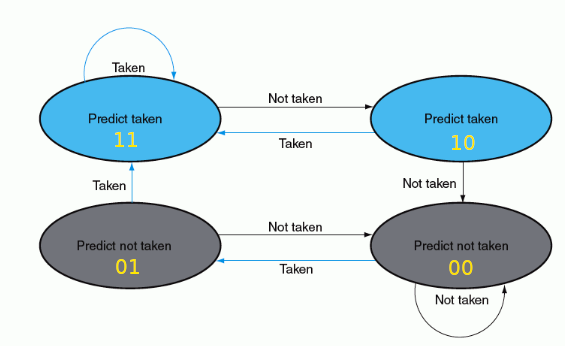
\includegraphics[width=0.7\linewidth]{imagenes/2bit-buffer-prediction}
		\caption{Maquinas de estados de predicción para un buffer de 2 bits}
		\label{fig:2bit-buffer-prediction}
	\end{figure}

	Las primeras implementaciones de esta técnica hacían uso de un único bit que se remplazaba cada vez que la predicción fallaba. En ciertos casos, la eficiencia de este método no era satisfactoria llegando a fallar completamente en otros (por ejemplo, si los saltos termina formando una secuencia intercalada de Taken y Not taken).
	
	\item \textbf{Branch Target Buffer (BTB)}: Es una caché en la que se almacena, en cada entrada, la dirección de la instrucción de control y la dirección de la instrucción que fue ejecutada después de resolver el branching.
	
	Cuando se fetchea una instrucción de control, se accede a esta caché usando el valor del program counter.
	\begin{itemize}
		\item Si el valor no está en el buffer, entonces se asume \textit{taken}.
		\begin{itemize}
			\item Si el resultado es \textit{Non-Taken} se acepta el delay en el pipeline y no se almacena nada en el BTB.
			\item Si el resultado es \textit{taken}, se ingresa el valor al BTB.
		\end{itemize}
		\item Si el valor se encuentra en el BTB, se aplica el campo de dirección de target almacenado.
		\begin{itemize}
			\item si el resultado es \textit{taken} no hay penalidad. No se guarda en el BTB ningún nuevo valor ya que el que está almacenado es el que nos sirve.
			\item Si el resultado es \textit{Non-taken}, guarda el nuevo valor en el BTB, luego de la penalidad correspondiente en el pipeline. 
		\end{itemize}
	\end{itemize}
\end{itemize}

\newpage
\section{Procesadores Superscalares}
Son procesadores que explotan la ejecución paralela de instrucciones para mejorar el rendimiento. Agrega más pipelines a la ejecución, lo que permite incrementar aún más la cantidad de instrucciones procesadas por ciclo de reloj.

Un problema es que los obstáculos estructurales quedan más expuestos. Cada etapa, ademas de lidiar con los data hazards de su propio pipeline, debe lidiar también con las mismas etapas del otro pipeline. 

Este tipo de procesadores analizan los binarios secuenciales de los programas y lo paralelizan eliminando esencialidad innecesaria. Por esta razón, los programas binarios deben ser vistos más como una especificación de lo que debe hacerse y no como lo que realmente sucede.

Más precisamente, un procesador superescalar implementa:

\begin{enumerate}
	\item Estrategias de fetch que permiten fetchear múltiples instrucciones mediante la predicción de resultados y saltos.
	\item Métodos para determinar dependencias de registros y mecanismos para comunicar esos valores cuando sea necesario durante la ejecución.
	\item Métodos para iniciar, o resolver, múltiples instrucciones en paralelo.
	\item Recursos para la ejecución en paralelo de varias instrucciones, incluyendo múltiples unidades funcionales de pipelines y jerarquías de memorias capaces de atender simultáneamente múltiples referencias a memoria.
	\item Métodos para manejar datos a través de instrucciones de lectura/escritura e interfaces de memoria que tengan en cuenta el comportamiento dinámico (y muchas veces impredecibles) de las jerarquías diseñadas.
	\item Métodos para actualizar los estados del proceso en el orden correcto (para mantener la apariencia de la ejecución en orden secuencial).
\end{enumerate}

\subsection{Dependencias de instrucciones}\label{sec:instructionLevelParalelism:dependenciaDeInstrucciones}
Por lo general, se interpreta el binario de un programa como un conjunto de bloques compuestos de instrucciones contiguas. Una vez que se fetchea un bloque, se sabe que todas sus instrucciones van a ser ejecutadas eventualmente. Cuando esto suceda, diremos que el bloque es iniciado en una \textbf{ventana de ejecución}.

Una vez que las instrucciones entran en esta ventana, son ejecutadas en paralelo teniendo en cuenta sus dependencias que pueden ser de control o datos. Las de control son generadas por condicionales y pueden ser resueltas/optimizadas con predicciones (Sección \ref{sec::branchPrediction}). 

Las \textbf{dependencias de datos} se da entre instrucciones que referencian el mismo espacio de memoria. En estos casos, si las instrucciones no se ejecutan en el orden correcto, puede haber errores en las operaciones. Pueden ser Verdaderas o Artificiales
\begin{itemize}
	\item \textbf{Dependencias verdaderas:} Cuando una instrucción debe leer un valor que todavía no fue generado por una instrucción previa (\textbf{Read after write hazard}).
	\item \textbf{Dependecias artificiales:} Resultan de instrucciones que deben escribir un nuevo valor en una posición de memoria pero debe esperar a que las instrucciones previas utilicen el valor actual (\textbf{Write after Read hazard}) o cuando varias instrucciones deben escribir la misma posición de memoria (\textbf{Write after Write hazard}).
	
	Estas dependencias son producidas por código no optimizado, por escasez de registros disponibles, por el deseo de economizar el uso de la memoria principal o por ciclos donde una instrucción puede colisionar consigo misma.
	
\end{itemize}


\subsection{Fetching and Decode}\label{ilp::superscalars::fetchDecode}
En los procesadores superescalares, una caché de instrucciones se usa para reducir la latencia y incrementar el ancho de banda del fetching. Esta caché está organizada en bloques o lineas que contienen varias instrucciones consecutivas y almacena el tipo de cada una de ellas (si es de control, de operación, de lectura de memoria, etc). 

El program counter se utiliza para determinar la posición de una instrucción en la caché.

\begin{itemize}
	\item Si se produce un hit, se fetchea el bloque de instrucciones y se suma al program counter el tamaño del bloque fetcheado.
	\item Si hay un miss, el caché pide la instrucción buscada en memoria y la copia.
	\item Se identifica el tipo de cada instrucción. Si alguna es de control, se realizan las predicciones usando alguno de los métodos mencionado en en la sección \ref{sec::branchPrediction}.
	\item Las instrucciones son decodificadas en  \textbf{tuplas de ejecución} que contienen la operación a ser ejecutada, las identidades de los elementos donde se encuentran los parámetros de entrada y donde deben guardase los resultados. 
	
	En el programa estático, las instrucciones utilizan los registros \textbf{lógicos} (los de la arquitectura). Por esta razón, cuando son decodificadas, se mapean (o renombran) a un registro físico y las dependencias artificiales se resuelven indicando a las instrucciones involucradas que usen distintos registros físicos (\textbf{Algoritmo de tomasulo}, sección \ref{ilp::tomasulo}).

	\item Una vez que todas las instrucciones asociadas a un registro físico son completadas (modifican el estado visible), se libera el registro para que pueda ser usado por otro bloque de instrucciones. 		
\end{itemize}

\subsection{Scoreboarding}
Cuando una instrucción es decodificada, se loguea en un archivo de registros llamado \textbf{scoreboard}. Éste se encarga de commitear, mandar a ejecutar y detectar dependencias. Cuando detecta que las instrucciones pueden leer sus operandos las manda a ejecutar. Si decide que no puede hacer esto, monitorea cada cambio del hardware hasta que los operandos necesarios estén disponibles.
Además, controla cuando una instrucción puede escribir sus resultados en el registro correspondiente. De esta manera, la detección de hazards y su resolución es centralizada en el scoreboard. 

Durante la ejecución, cada instrucción pasa por cuatro etapas:

\begin{enumerate}
	\item \textbf{Issue:} Si hay una unidad funcional libre para la instrucción y ninguna otra instrucción activa necesita escribir en el registro destino, el scoreboard la envía a esta unidad y actualiza su estado interno. Si hubiese otra instrucción que necesita del mismo registro, entonces se bloquea (\textit{stall}) hasta que todos los obstáculos hayan sido resueltos.
	
	Cuando esta etapa se bloquea \textit{stall}, el buffer de Fetching también entra en este estado cuando se llena.
	
	\item \textbf{Lectura de operandos:} Un operando se encuentra disponible si ninguna instrucción activa emitida anteriormente necesita escribirlo. Cuando los operandos fuentes están habilitados, el scoreboard le dice a la unidad funcional que proceda a leerlos desde los registros y comience la ejecución. De esta forma se  evitan los RAW hazards que, como se resuelven dinámicamente, permiten que las instrucciones sean ejecutadas fuera de orden.
	
	\item\textbf{Ejecución:} Las unidades funcionales comienzan la ejecución después de haber recibidos todos los operandos. Cuando el resultado está listo, lo notifica al scoreboard.
	
	\item\textbf{Escritura de resultado:} Una vez que el scoreboard recibe la notificación, chequea por WAR hazards. Si los encuentra, bloquea la escritura de la instrucción hasta que estos son resueltos.
\end{enumerate}

\paragraph{Desventajas de este método}
\begin{itemize}
	\item No puede aprovechar el forwarding de datos porque considera que un operando solo está listo cuando fue escrito en registro.
	\item El scoreboard controla el progreso de una instrucción comunicándose con las unidades funcionales. Al haber un numero limitado de buses de operandos y resultados, debe asegurarse que el número de unidades funcionales habilitadas para proceder no excedan estos recursos.
\end{itemize}
\subsection{Tomasulo}\label{ilp::tomasulo}
El algoritmo de Tomasulo crea un scheduling dinámico que permite ejecutar instrucciones fuera de orden y habilita el uso de múltiples unidades de ejecución. Para lograr esto necesita:
\begin{itemize}
	\item Mantener un ``link'' entre el productor de un dato con su(s) consumidor(es).
	\item Mantener las instrucciones en espera hasta que estén listas para ejecución.
	\item Saber cuando sus operandos están listos (``Ready'').
	\item Despachar (``dispatch'') cada una de ellas a su Unidad Funcional correspondiente ni bien todos sus operandos estén listos.
\end{itemize}

\paragraph{Register Renaming:} El primer ítem se logra asignando a cada registro un alias. Para eliminar los WAR y WAW hazards, se utiliza una tabla llamada \textbf{Register Alias Table} que asocia un tag con cada operando de una operación.

\paragraph{Register Station (RS):} Una vez realizado el renombre se le asigna, a la instrucción, un RS. Un RS es un subsistema de hardware compuesto de bancos de registros internos que se encarga de mantener las instrucciones en espera hasta que estén listas para ser ejecutadas. Éste chequea constantemente por la disponibilidad de los operandos de la instrucción. Para cada uno de ellos cuyo valor no esté disponible, el RS, guarda el \textit{tag} que se le asignó en el paso anterior.

Cada vez que una unidad de ejecución pone disponible un operando, transmite el \textbf{tag} asociado al mismo junto con su valor a todas las RS. Cuando una instrucción tiene todos sus operandos disponible, el RS espera a que la unidad funcional asociada a ella esté libre y luego la despacha.

\paragraph{Common Data Bus}: Es un datapath que cruza la salida de las unidades funcionales y atraviesa las RS, los Floating Point Buffers, los Floating Points Registers y el Floating Point Operations Stack. Se usa para realizar el broadcast de los resultados al finalizar cada operación.

\paragraph{Pseudocodigo:}
Cada Registro contiene un tag que indica el último escritor en el registro.

\begin{algorithmic}
	\If{RS tiene recursos disponibles antes del renaming}
	\State{Se inserta en la RS la instrucción y los opernados renombrados (valor fuente / tag)}
	\State{Se renombra si y solo si la RS tiene recursos disponibles.}
	\Else
	\State{stall}
	\EndIf
	\While{esté en la RS, cada instrucción debe}
	\State{Mirar el tráfico por el \textbf{Common Data Bus (CDB)} en busca de \textbf{tags} que correspondan a sus Operandos fuente.}
	\State{Cuando se detecta un \textbf{tag}, se graba el valor de la fuente y se mantiene en RS.}
	\State{Cuando ambos operandos están disponibles, la instrucciónn se marca \textbf{Ready} para ser despachada}
	\If{Unidad Funcional disponible}
	\State{Se depscacha la instrucción a esa unidad funcional}
	\EndIf
	\If{Finalizada la ejecución de la instrucción}
	\State{La unidad funcional pone el valor correspondiente al \textbf{tag} en el \textbf{CD} (\textbf{tag broadcast})}
	\If{El archivo de registros está conectado al CDB}
	\If{tag del Archivo de Registro $==$ tag broadcast}
	\State{Registro = valor broadcast}
	\State{bit de validez = '1'}
	\State{Recupera \textbf{tag} renombrado}
	\State{No queda copia válida del tag en el sistema}
	\EndIf
	\EndIf
	\EndIf
	\EndWhile
\end{algorithmic}


\subsection{Ejecución de instrucciones}
\subsubsection{Interrupciones}
Existen dos tipos de interrupciones:
\begin{itemize}
	\item \textbf{Excepciones} (o trampas): Se generan cuando se produce un error durante la ejecución o el fetching de ciertas instrucciones. Por ejemplo, opcodes ilegales, errores numéricos o page faults.
	\item \textbf{Interrupciones externas}: Son causadas por instrucciones específicas y dispositivos externos qué están ejecutando algún proceso. Por ejemplo las interrupciones generadas por los dispositivos de entrada/salida (mouse, teclados, pantallas), timers, etc.
\end{itemize}

Cuando ocurre una interrupción, el software o el hardware (o una combinación de ambos) guardan el estado del proceso interrumpido. Este estado consiste, generalmente, del program counter, los registros y la memoria.

\paragraph{Interrupción precisa:} Una interrupción es precisa si el estado guardado es consistente con la arquitectura secuencial del modelo. Osea se debe cumplir que:
\begin{enumerate}
	\item Todas las instrucciones previas a la indicada por el program counter deben haber sido ejecutadas y deben haber modificado el estado del proceso correctamente.
	\item Ninguna de las instrucciones siguientes a la indicada por el program counter debe haber sido ejecutadas ni deben haber modificado el estado del proceso.
	\item Si la interrupción es causada por una excepción en una instrucción del programa, entonces el program counter guardado debe apuntar a la instrucción interrumpida.
\end{enumerate}

Si el estado guardado es inconsistente con el modelo de arquitectura secuencial y no satisface estas condiciones entonces la interrupción es \textbf{imprecisa}. 

\subsubsection{In-Order Instruction Completion}
Las instrucciones modifican el estado del proceso solo cuando se sabe que todas las instrucciones previas están libres de excepciones. Para asegurar esto se utiliza un registro llamado ``result shift register'' que contiene una tabla de $n$  entradas ($n$ la longitud del pipeline más largo). Una instrucción que toma $i$ ciclos de reloj, reserva la $i$-ésima entrada de la tabla y en cada ciclo se la desplaza una posición hacia abajo.
\begin{figure}[ht]
	\centering
	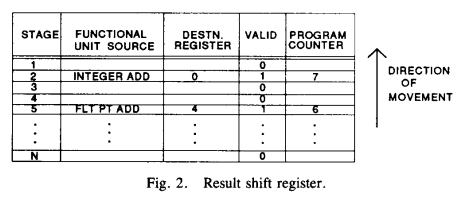
\includegraphics[width=0.5\linewidth]{imagenes/shift-register}
	\caption{Result Shift Register}
	\label{fig:shiftregister}
\end{figure}

Si la $i$-ésima entrada contiene información valida entonces se pausa la instrucción. En el próximo ciclo, se re chequea si la entrada está libre y se realiza el movimiento.

Para evitar que una instrucción más corta se complete antes que otra de mayor longitud (cuando este es el orden deseado) se rellenan con información invalida todas las entradas anteriores que no fueron reservadas. De esta forma, la nueva instrucción es pausada hasta el próximo ciclo de reloj.

\subsubsection{Reorder-Buffer}
La principal desventaja del método anterior es que instrucciones rápidas serán retenidas a pesar de no tener dependencias.

Para resolver este problema se agrega un \textbf{reorder buffer} que indica el orden en el que las instrucciones deben modificar el estado visible. Entonces se permite que las instrucciones terminen en cualquier orden pero se les asigna un tag que cumple con el objetivo mencionado. Cuando son completadas, se las almacena en la entrada indicada (por el tag) del buffer.

\begin{figure}[ht]
	\centering
	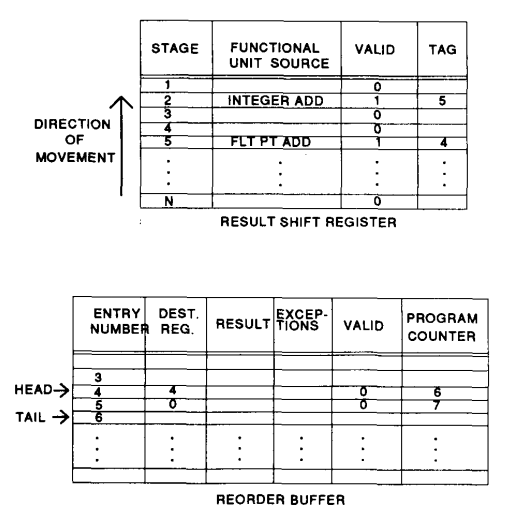
\includegraphics[width=0.5\textwidth]{imagenes/reorder-buffer}
	\caption{Reorder buffer}
	\label{fig:reorder-buffer}
\end{figure}

El buffer contiene un puntero a la entrada que corresponde a la próxima instrucción a ser ejecutada. Cuando dicha entrada contenga información válida, se  chequea si hubo excepciones. Sí no las hubo, se modifican los registros/memoria necesarios y se mueve el puntero a la próxima entrada. Sino, se emite la excepción y se invalidan todas las entradas posteriores.

En algunos casos, la dependencia entre instrucciones requiere el uso de valores que todavía no fueron escritos en los registros. Para conseguirlos es necesario acceder al buffer de reordenamiento, lo que agrega latencia y complejidad a la ejecución.

\paragraph{History Buffer:} Una solución posible es dejar que las instrucciones modifiquen los registros cuando son completadas, pero que se guarden los valores previos en un buffer que permita recuperar estos datos en el caso de una excepción.

En este caso, si ocurre una excepción, se debe recorrer el history buffer para poder recuperar un estado preciso.

\paragraph{Future File:} Otra solución es mantener dos archivos de registros. Uno que se actualice en el orden especificado por el programa (\textbf{Architectural File}). Y otro que se actualiza apenas se completa una instrucción (\textbf{Future File}).

Si ocurre una excepción simplemente se debe mostear el Architecture File para conseguir un estado preciso. Sin embargo, hay que copiarlo al future file para restaurar el estado del sistema.

\paragraph{Checkpointing:} Cuando se predice el resultado de una instrucción de control, se guarda el estado del future file (\textbf{checkpoint}). Si al ejecutarla, la predicción resulta ser errónea entonces solo hay que copiar la información del checkpoint en el future file para recuperar el estado del sistema y comenzar de nuevo en la instrucción correcta.  
